\input /Users/davidmcallester/ICloude/tex/SlidePreamble
\input /Users/davidmcallester/ICloude/tex/preamble


\begin{document}

{\Huge

  \centerline{\bf TTIC 31230, Fundamentals of Deep Learning}
  \bigskip
  \centerline{David McAllester, Autumn 2020}
  \vfill
  \centerline{\bf Generative Adversarial Networks (GANs)}
  \vfill
  \centerline{\bf A Timeline of GAN Development}
\vfill
\vfill


\slide{GANs}

\begin{eqnarray*}
\Phi^* & = & \argmax_\Phi\;\;\min_\Psi\;E_{\tuple{i,y} \sim \tilde{p}_\Phi}\;-\ln P_\Psi(i|y)
\end{eqnarray*}

\vfill
$$\Phi^* = \argmax_\Phi\;\;\min_\Psi\;\left\{\begin{array}{ll} & E_{y \sim \popd}\;-\ln P_\Psi(1|y) \\ \\ + &  E_z\;-\ln P_\Psi(-1|y_\Phi(z)) \end{array}\right.$$

\slidetwo{Generative Adversarial Nets}{Goodfellow et al., June 2014}
\centerline{\includegraphics[width = 9in]{\images/GAN2014}}
The rightmost column (yellow boarders) gives the nearest neighbor in the training data to the adjacent column.

\slidetwo{Unsupervised Representation Learning ... (DC GANS)}
{Radford et al., Nov. 2015}

\centerline{\includegraphics[width = 9in]{\images/GANDCa}}

\slidetwo{Unsupervised Representation Learning ... (DC GANS)}
{Radford et al., Nov. 2015}

\centerline{\includegraphics[width = 9in]{\images/ImageFeatures}}

\slide{Interpolated Faces}

[Ayan Chakrabarti, January 2017]

\centerline{\includegraphics[height = 4.5in]{\images/interp}}

\slide{Conditional GANS}
In the conditional case we have a population distribution over pairs $\tuple{x,y}$.

\vfill
For conditional GANs we have a generator $p_\Phi(y|x)$ and a discriminator $P_\Psi(i|x,y)$
where $i = 1$ if $y$ the real ``label'' for $x$ and $-1$ if $y$ is generated from $x$.

{\color{red} $$\Phi^* = \argmax_\Phi\;\;\min_\Psi\;E_{\tuple{x,y,i} \sim \tilde{p}_\Phi}\;-\ln P_\Psi(i|x,y)$$}

\slidetwo{Image-to-Image Translation (Pix2Pix)}
{Isola et al., Nov. 2016}

We assume a corpus of ``image translation pairs'' such as images paired with semantic segmentations.

\centerline{\includegraphics[width = 8.0in]{\images/cGAN0}}


\slide{Adversarial Discrimination as an Additional Loss}

$${\color{red} \Phi^* = \argmin_\Phi\;E_{(x,y) \sim \popd}\;\; ||y- y_\Phi(x)||^2\; + \; \lambda\; {\cal L}_{\mathrm{Discr}}(\Phi)}$$

\vfill
$${\cal L}_\mathrm{Discr}(\Phi) = \max_\Psi \;E_{x,y,i \sim \tilde{p}_\Phi}\; \ln P_\Psi(i|y,x)$$

\slide{Discrimination as an Additional Loss}

{\huge
$$\begin{array}{lrcl}
\mathrm{L1:} & \Phi^* & = & \argmin_\Phi\;E_{(x,y) \sim \popd}\;\; ||y - y_\Phi(x)||_1 \\
\\
\\
\mathrm{cGAN:} & \Phi^* & = & \argmin_\Phi\;{\cal L}_{\mathrm{Discr}}(\Phi) \\
\\
\\
\mathrm{L1 + cGAN:} & \Phi^* & = & \argmin_\Phi\;E_{(x,y) \sim \popd}\;\; ||y - y_\Phi(x)||_1\; +\; \lambda\; {\cal L}_\mathrm{Discr}(\Phi)
\end{array}$$
}


\slidetwo{Image-to-Image Translation (Pix2Pix)}
{Isola et al., Nov. 2016}

\centerline{\includegraphics[height = 4.5in]{\images/cGAN1}}

\slide{Arial Photo to Map and Back}

\centerline{\includegraphics[width = 8.0in]{\images/cGAN2}}

\slidetwo{Unpaired Image-to-Image Translation (Cycle GANs)}{Zhu et al., March 2017}

We have two corpora of images, say images of zebras and unrelated images of horses, or photographs and unrelated paintings by Monet.

\vfill
We want to construct translations between the two classes.

\centerline{\includegraphics[width = 8.0in]{\images/Cycle2}}

\slide{Cycle Gans}

\centerline{\includegraphics[width = 11.0in]{\images/Cycle3}}

\slide{Cycle Gans}

\centerline{\includegraphics[width = 6.0in]{\images/Cycle4}}

\slidetwo{Unsupervised Machine Translation (UMT)}
         {Lample et al, Oct. 2017, also Artetxe et al., Oct. 2017}


In unsupervised machine translation the cycle loss is called {\bf back-translation}.

\slidetwo{Feature Alignment by Discrimination}{Text to Speech (Saito et al. Sept. 2017)}

\centerline{\includegraphics[width = 2.0in]{\images/Txt2spchGAN}}

\vfill
Minimum Generation Error (MGE) uses {\color{red} perceptual distortion} ---
a distance between the feature vector of the generated sound wave and the
feature vector of the original.

\vfill
{\color{red}Perceptual Naturalness} can be enforced by a feature discrimination loss.

\slidetwo{Adversarial Discriminative Domain Adaptation}{Tzeng et al. Feb. 2017}

\centerline{\includegraphics[width = 4.0in]{\images/AdvDomainAdapt}}

A feature discrimination loss can be used to align source and target features.

\slide{Progressive GANs}

\centerline{Progressive Growing of GANs, Karras et al., Oct. 2017}

\centerline{\includegraphics[height = 4.5in]{\images/GANproga}}

\slide{Progressive GANs}

\centerline{\includegraphics[height = 4.5in]{\images/GANprogb}}

\slide{Early GANs on ImageNet}

\centerline{\includegraphics[height = 4.5in]{\images/BadGAN}}

\slide{BigGans}
\centerline{Large Scale GAN Training, Brock et al., Sept. 2018}
\centerline{\includegraphics[width = 9in]{\images/GANclass}}

\vfill
This is a class-conditional GAN --- it is conditioned on the imagenet class label.

\vfill
This generates 512 X 512 images without using progressive training.

\slide{StyleGANs}
{\Large A Style-Based Generator Architecture for Generative Adversarial Networks, Karras et al., Dec. 2018}

\centerline{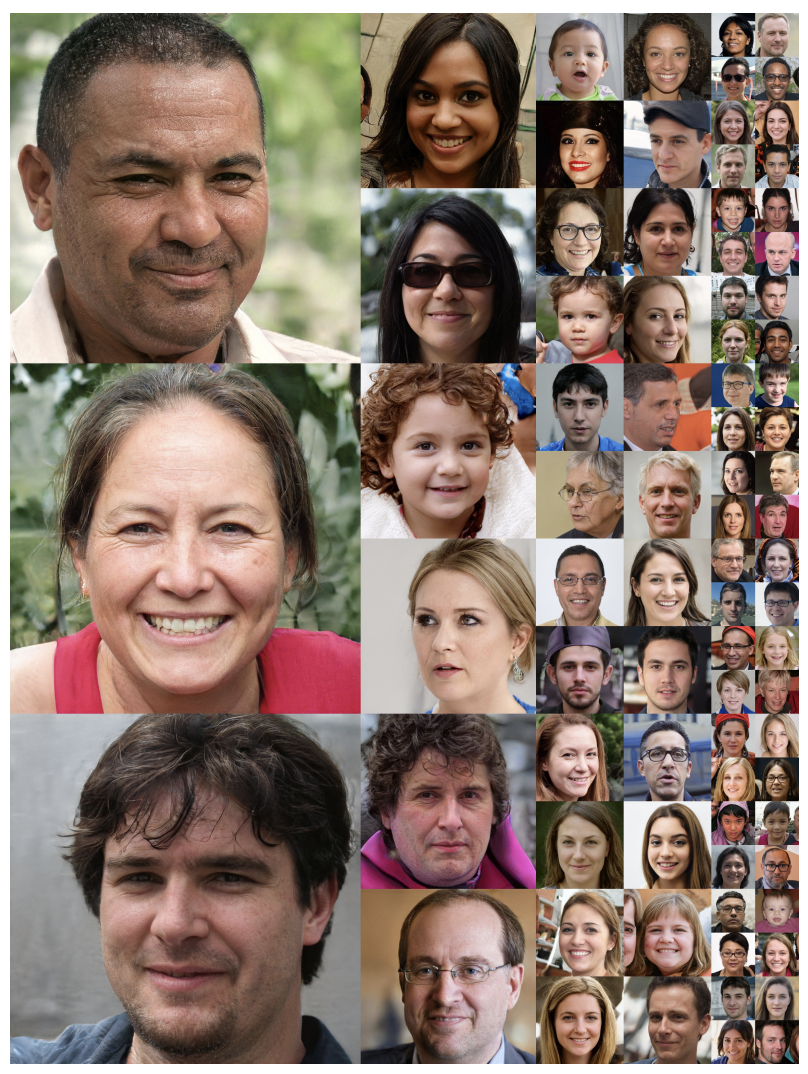
\includegraphics[height= 4.8in]{\images/Style1}}

\slide{StyleGans: Architecture}

\centerline{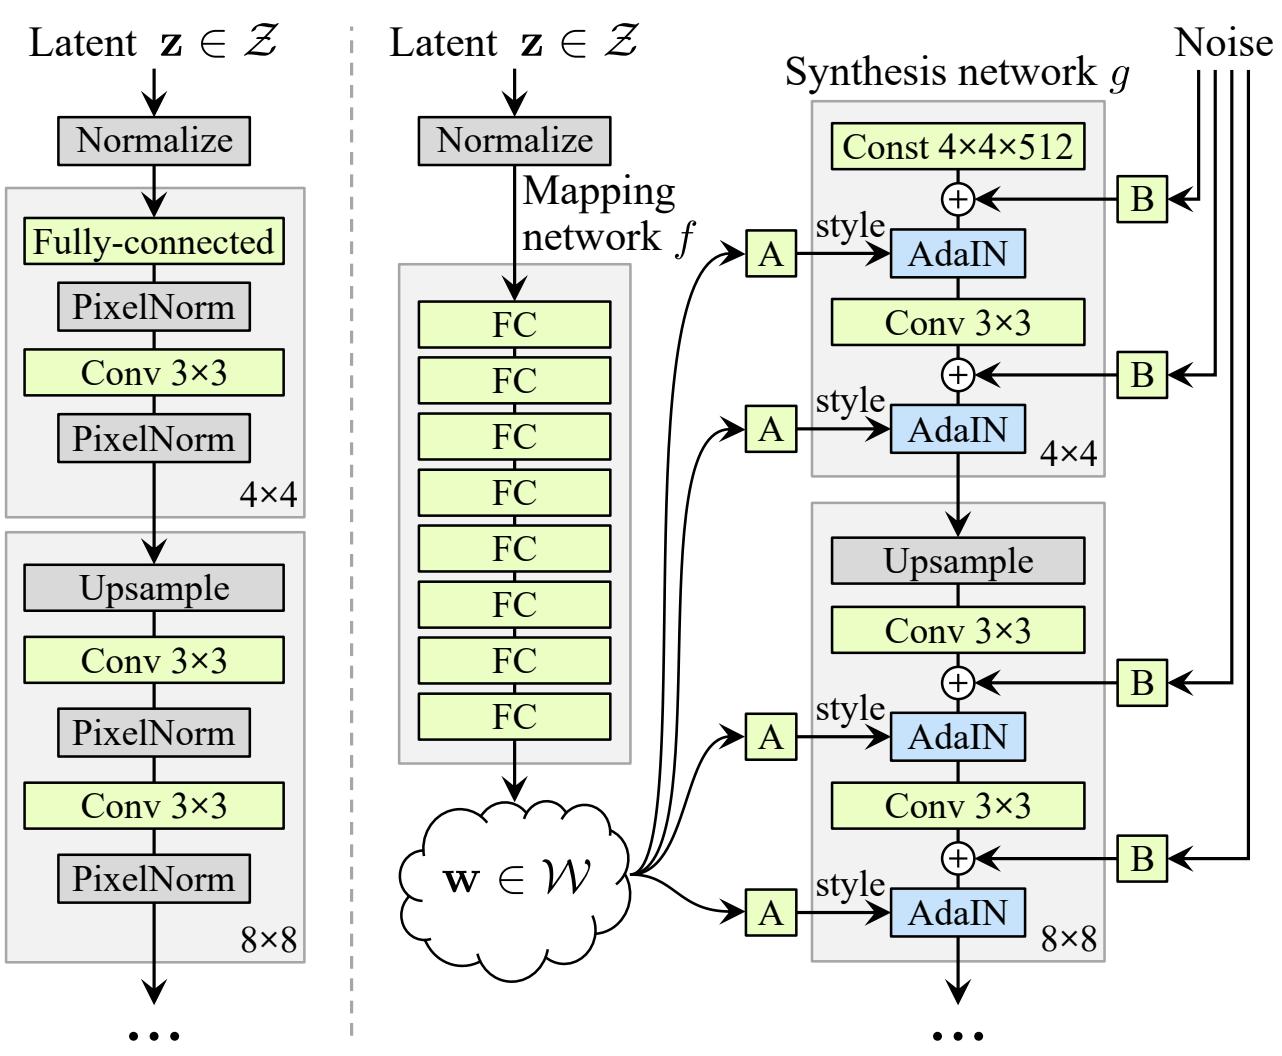
\includegraphics[height= 5.2in]{\images/StyleArch}}

\slide{StyleGans: Style Transfer}

\centerline{\includegraphics[height= 5.2in]{\images/Style2}}

\slide{StyleGans: Noise Variation}

\centerline{\includegraphics[height= 5.2in]{\images/Style3}}

\slide{StyleGANS2}

StyleGan2 appeared in December of 2019 with significant improvements.

\vfill
It was demonstrated to work on many classes of images, not just faces.

\slide{Projecting Images into Latent Space}

Given an image, can we find a noise vector (a latent vector) that generate a close approximation of
the given image.  Can we invert the generator?

\vfill
This appears to be possible with StyleGAN2 but not with the original even though StyleGAN2 produces better images.

\vfill
By measuring the match between an image $y$ and $g(g^{-1}(y))$ we can determine whether $y$ was generated by StyleGAN2.

\slide{GANs for Pretraining}

A main motivation for distribution modeling is to provide pre-trainined models that can be used in downstream tasks.

\vfill
This has proved very effective in natural language processing.

\vfill
To date GANs have not provided competative pretraining for downstream applications other than image generation.

\slide{END}

}
\end{document}
